\section{Motivation}\label{sec:motivation}
Generally, snow metamorphoses via one of two processes: kinetic or equilibrium metamorphism. Efforts to simulate this behavior use a range of approaches and frameworks and include purely statistical modules, continuum bulk property formulations, and complete numerical 3D constructs. Despite the wide spectrum of snow and avalanche models that exist, currently there is no unified modeling effort to allow true collaboration across models as scales. Given the broad range modeling approaches for snow and avalanche research (see Section \ref{sec:background}) a new paradigm is needed for simulations that fosters rapid development and collaboration.\authorcorrespond This paper aims to demonstrate the capabilities of the open-source Multiphysics Object Oriented Simulation Environment (MOOSE; \url{www.moooseframework.org}) as a framework for future snow and avalanche model development.

MOOSE is a finite-element framework that aids in application development by harnessing state-of-the-art fully-coupled, fully-implicit multiphysics solvers while providing automatic parallelization, mesh adaptivity, and an ever expanding set of physics modules including solid mechanics, phase-field, Navier-Stokes, and heat conduction. MOOSE natively supports multi-scale models allowing to couple MOOSE-based applications, thus fostering collaborations \citep{gaston2014physics}. Finally, MOOSE follows a rigorous and development strategy that ensures software quality at both the framework and application level \citep{gaston2014continous}.

This paper briefly demonstrates the capabilities of MOOSE by:
\begin{enumerate}\setlength{\itemsep}{0pt}
\item developing a meso-scale continuum model for heat-condition, named Ibex, following the methods of \citet{slaughter2010numerical} in Section \ref{sec:ibex},
\item developing a snow micro-structure model (Pika) based on the work of \citet{kaempfer2009phase} in Section \ref{sec:pika}, and
\item coupling the two models together into a single, multi-scale simulation (Yeti) in Section \ref{sec:yeti}.
\end{enumerate}

The purpose of the work is not to provide a validated, fully-operational model for snow, but to take existing modeling approaches and re-implement them using a single framework to demonstrate the capabilities of MOOSE. The tools developed here are the basis for a completely new approach to modeling snow, an approach that aims to bring groups together to build a myriad of different, open-source simulation tools utilizing using a common framework to allow for coupling and co-development.


\section{Background}\label{sec:background}
Modeling the thermal behavior of snow is not a new endeavor; \citet{lachapelle1960critique} cites a paper from 1892 that examined temperature profiles of snow. A significant amount of work has examined snow using a continuum mechanics theory of mixtures (e.g., \citet{adams1989constitutive, brown1999mixture}.  Using a thermal non-equilibrium approach, \citet{bartelt2004nonequilibrium} indicated that temperature differences between the pore air and ice particles and inter-facial heat exchange between snow crystals played a significant role in determining the temperature profile. Perhaps the most comprehensive model developed to date is the SNOWPACK model \citep{bartelt2002physical, lehning2002physiCal, lehning2002physicalb}, that accounts for heat transfer, water transport, vapor diffusion, and mechanical deformation.  Research conducted in an attempt to validate the SNOWPACK model yielded reasonable results, yet \citet{fierz2001assessment} encouraged additional work regarding the initial stage of snow metamorphism, specifically the processes involving particles changing to small faceted or rounded crystals. \citet{miller2009microstructural} provided a unique approach for modeling this transition. They were able to develop a model capable of faceted growth, but the model is limited in a number of ways, including an assumed spherical geometry.

Recent approaches to modeling the snowpack are based on the 3D images of the snow micro-structure.  One notable article by \citet{kaempfer2005microstructural} utilized X-ray micro-tomography ($\mu$-CT) to build a 3D image of a snow sample to which a finite element model was applied for modeling the heat transfer through the sample. \citet{kaempfer2009phase} demonstrated that phase-field methods may be applied to snow metamorphism and concludes that with the model ``snow metamorphism can be studied in details not possible heretofore.'' This approached is used as the staring point for the work presented in this paper.


\section{Ibex: Meso-scale model}\label{sec:ibex}
The meso-scale model presented here is comprised of a single relationship, the heat-equation:
\begin{equation}\label{eq:meso}
\rho c_p \frac{\partial{T}}{\partial t} = \nabla \cdot k_{eff} \nabla T + s,
\end{equation}
where $t$ is time, $T$ is temperature, $s$ a heat source term, and the material properties $\rho$, $c_p$, and $k_{eff}$ are the bulk density, specific heat, and thermal conductivity for snow. The model developed includes incoming shortwave radiation that is absorbed within the snow (i.e., the $s$ source term in Eq. \eqref{eq:meso}), including absorption that differs with wavelength as detailed by \citet[][Ch.4]{slaughter2010numerical}. On the surface the effects of incoming and out going long-wave radiation as well as sensible and latent heat are included as detailed in \citet{slaughter2010numerical}.

To demonstrate the accuracy of the model, Exp. \#2 of \citet{morstad2007experimental} was reproduced using a 1D Ibex simulation. The simulation was setup using the parameters detailed in \citet[][Ch.4]{slaughter2010numerical} including incoming short- and long-wave radiation set to \unitfrac[650]{W}{m\textsuperscript{2}} and \unitfrac[235]{W}{m\textsuperscript{2}}, respectively and the albedo in the visible, near-infrared, and short-wave infrared defined as 0.94, 0.80, and 0.59, respectively.

Fig. \ref{fig:ibex_1d} includes the simulation results and a comparison with the experimental data of \citet{morstad2007experimental} after 8 hours; qualitatively the 1D Ibex model is capable capturing the general trend of experimental data. Providing the complete details and fine tuning and validated the parameters for Ibex is beyond the scope of this demonstration paper.



Since, Ibex was built using MOOSE, it is dimension agnostic, thus the same code that produced the 1D results above is also capable of running in 3D with adaptive meshing, as shown in Fig. \ref{fig:ibex_3d}, without altering anything except the input file. This simulation uses the same input parameters as mentioned above, except applies the incoming short-wave irradiance as function of space and time. This demonstrates the flexibility of MOOSE-based application to build flexible and extensible applications, which will be further demonstrated in the next section.


\begin{figure}[t]
  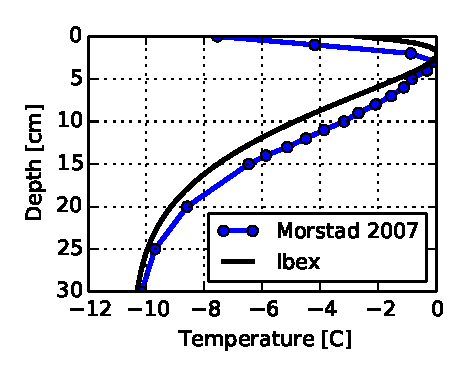
\includegraphics[width=3.125in]{figures/ibex.pdf}
  \caption{Comparison of experimental data and 1D Ibex simulation.}
  \label{fig:ibex_1d}
\end{figure}

\begin{figure}[!ht]
  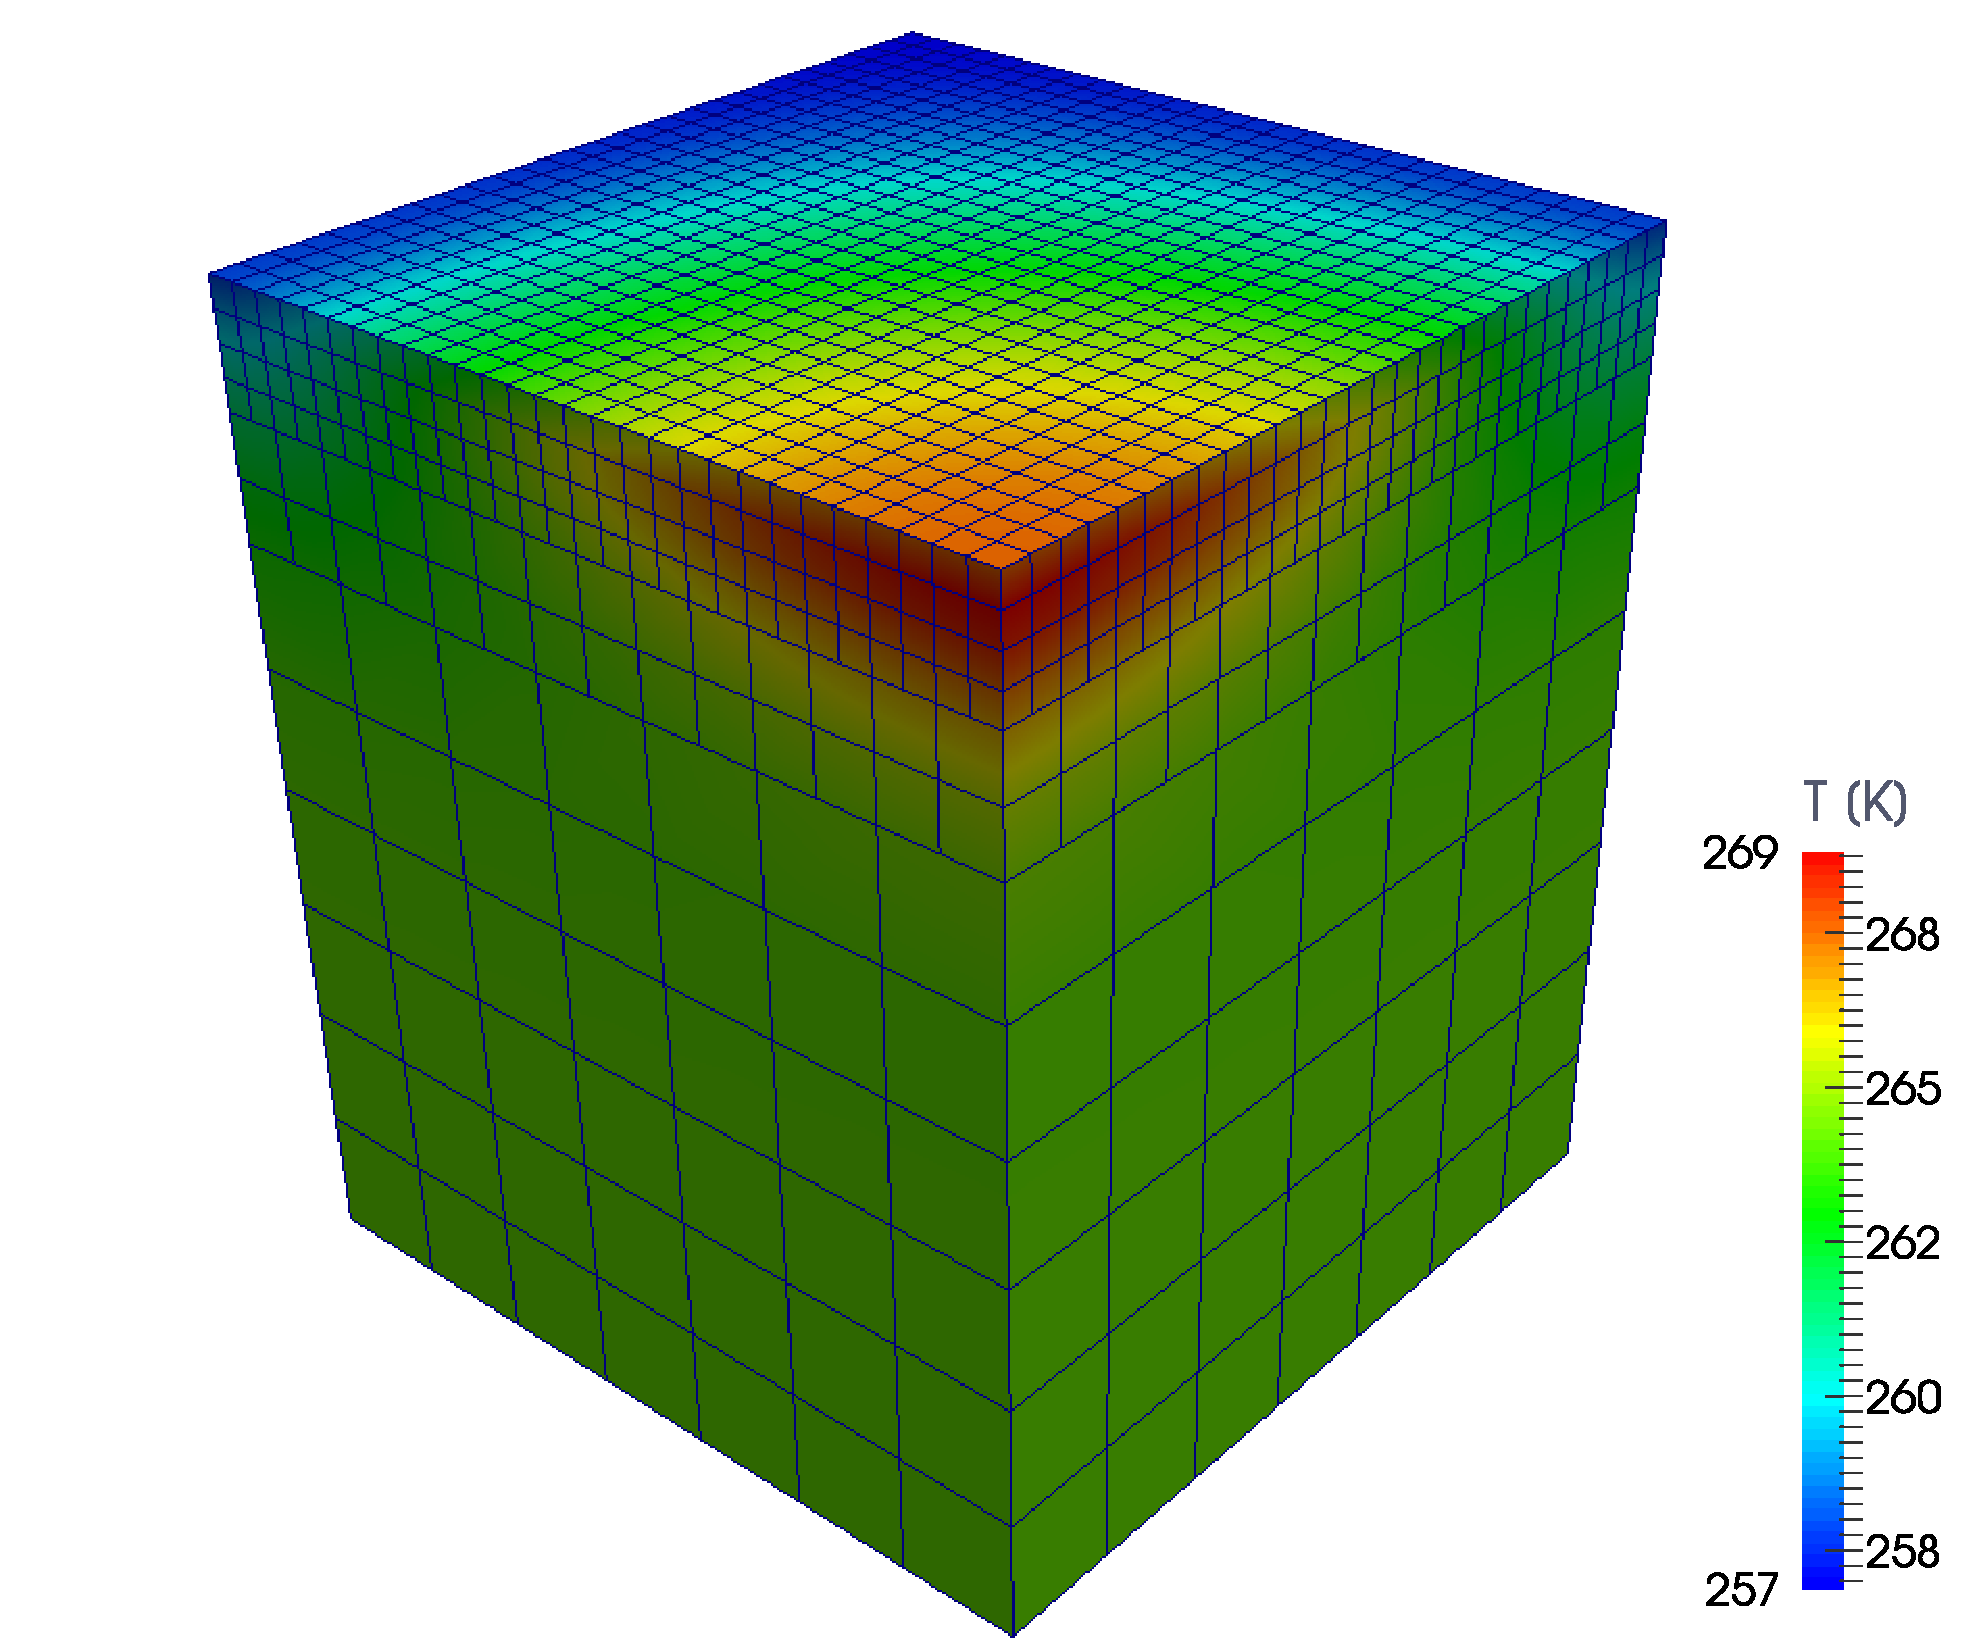
\includegraphics[width=\linewidth]{figures/ibex3d.pdf}
  \caption{Demonstration of 3D Ibex simulation with spatial and temporal varying incoming short-wave irradiance.}
  \label{fig:ibex_3d}
\end{figure}



\section{Pika: Micro-structure Model}\label{sec:pika}
A phase-field micro-structure model based on the work of \citet{kaempfer2009phase} was developed that tracks heat and mass transfer and includes sublimation and deposition of water-vapor. The MOOSE framework includes a phase-field module \citep{tonks2012object}, thus making the this approach a natural choice.

The model is comprised of three relationships: the phase-field, heat, and mass transport equations. The phase-field equation, as defined in Eq. \eqref{eq:phase}, allows the phase transition from ice to pore space to be modeled as a continuous, smooth variable allowing for complex geometries to be captured with a arbitrary finite element grid.
\begin{equation}\label{eq:phase}
\tau \frac{\partial \phi}{\partial t} = W^2 \nabla^2 \phi +(\phi-\phi^3)+\lambda[u-u_{eq}](1-\phi^2)^2,
\end{equation}
where $\phi$ is the phase-field variable (1 for ice; -1 for pore), $t$ is time, $\tau$ is the phase-field relaxation time, $W$ is the interface thickness, $\lambda$ is the phase-field coupling constant, $u$ is the dimensionless vapor concentration, and $u_{eq}$ is the dimensionless vapor concentration at equilibrium. The $\tau$ and $\lambda$ terms dictate kinetics of the micro-structure evolution and are detailed by \citet{kaempfer2009phase}.

The heat equation is given in Eq. \eqref{eq:heat}, which includes a forcing term that accounts for the gain or loss of heat due to phase change.
\begin{equation}\label{eq:heat}
C(\phi)\frac{\partial T}{\partial t} = \nabla \cdot [K(\phi) \nabla T] + \frac{L_{sg}}{2}\frac{\partial \phi}{\partial t},
\end{equation}
where $T$ is temperature, $C$ and $K$ are the phase-field adjusted heat capacity and thermal conductivity, respectively, and $L_{sg}$ is the latent heat of sublimation.

Equation \ref{eq:vapor} is the mass-transport equation that models the diffusion of vapor in the pore space.
\begin{equation}\label{eq:vapor}
\frac{\partial u}{\partial t} = \nabla \cdot[ D(\phi) \nabla u] - \frac{1}{2}\frac{\partial \phi}{\partial t},
\end{equation}
where $D$ is the phase-field adjusted vapor diffusion coefficient.

The model developed here---Pika---generally follows the formulation presented by \citet{kaempfer2009phase} with a few notable exception: (1) Pika utilizes a finite element solution as opposed to a finite difference and (2) Pika allows the interface kinetic coefficient ($\beta$) and capillary length ($d_0$), which dictate the $\tau$ and $\lambda$ terms of Eq. \eqref{eq:phase}, to vary with temperature whereas \citet{kaempfer2009phase} held these terms constant.

Fig. \ref{fig:bubble} shows the results of a benchmark problem modeled by \citet{kaempfer2009phase} and reproduced here for comparison. The problem is based on experiments of a bubble inside a block of ice having a \unit[5]{mm} square cross section that is subjected to to various temperature gradients \citep{nakaya1956technical, stehle1965technical}. The results shown here are for a gradient of \unitfrac[543]{K}{m} and match well with those reported by \citet{kaempfer2009phase}. The Pika model exhibited an average interface velocity of \unitfrac[3.73e-9]{m}{s} at \unit[7200]{s}, which is similar to those reported \citet{kaempfer2009phase}.


Utilizing the simulation settings similar to the benchmark problem a simulation was performed on a $\mu$-CT scanned cross-section of snow measuring \unit[5]{mm} square. This sample was obtained at the Subzero Science and Engineering Research Facility at Montana State University. The simulation was subjected to a temperature gradient of \unitfrac[250]{K}{m} for approximately eight hours.

As shown in Fig. \ref{fig:keff}, during the simulation the effective thermal conductivity ($k_{eff}$) was computed in the vertical (y) and horizontal directions (x), which were on the order of \unitfrac[1.2]{W}{mK}, which is on the upper limit of what is expected for snow \citep{sturm1997thermal}. The $k_{eff}$ value accounts for heat transfer by diffusion only, thus in essence is an indicator of the conduction through the ice matrix.

Fig. \ref{fig:snow2d:diff} includes the raw snow image overlaid with the areas that observed sublimation (hot colors) and deposition (cold colors) and Fig. \ref{fig:snow2d:grains} snow the temperature field at the end of the simulation as well as the ice grain locations at the beginning and end of the simulations.

\begin{figure}[t]
  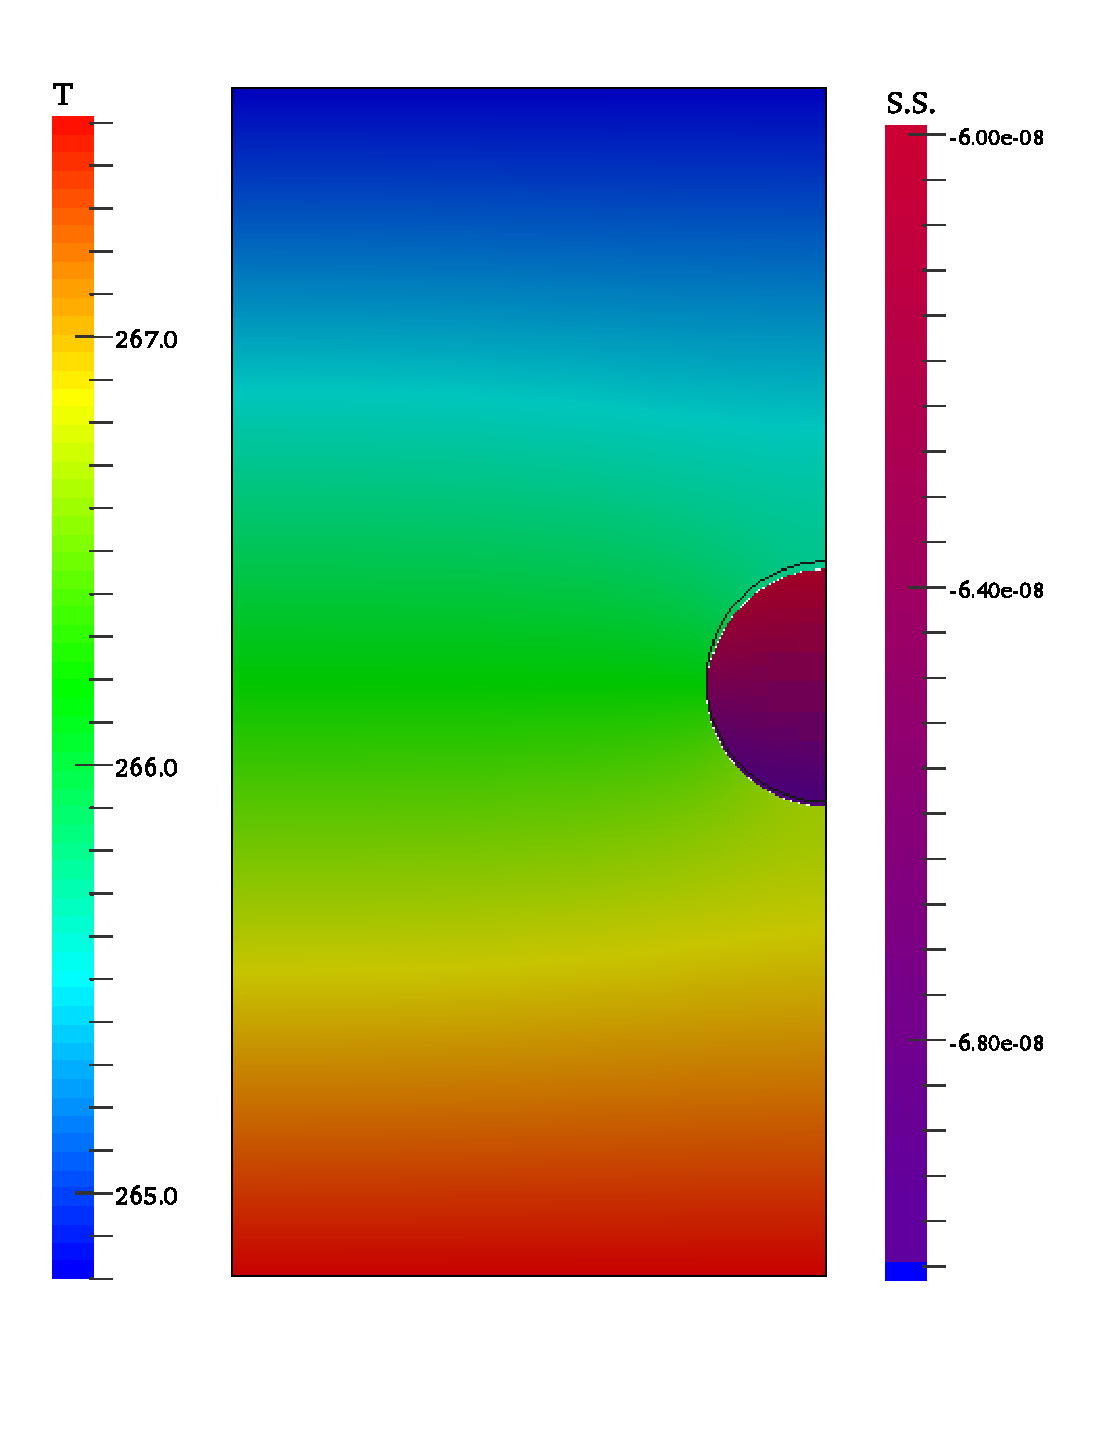
\includegraphics[width=\linewidth]{figures/bubble.pdf}
  \caption{Benchmark problem of bubble within \unit[5]{mm} cross section of ice; temperature (T) reported in \unit[]{K} and supersaturation (S.S.) in \unitfrac[]{kg}{m$^3$}.}
  \label{fig:bubble}
\end{figure}


\begin{figure}
  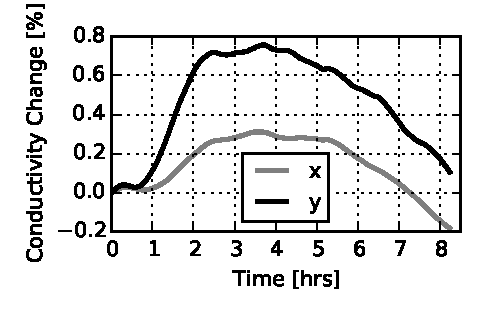
\includegraphics[width=\linewidth]{figures/pika_keff.pdf}
  \caption{Percent change in effective thermal conductivity in the vertical (y) and horizontal directions (x) during the simulations.}
  \label{fig:keff}
\end{figure}



The $k_{eff}$ results are of particular interest, during the first few hours of the simulation both values increase, with the vertical direction increase at a greater rate. Then both begin to decrease at a similar rate after about four hours. There may be many explanations for this behavior. This decrease may be indiciative of the pore space beginning to align in the direction of the gradient, which is expected, thus reducing the ice connectivity. However, considering the simplicity of the phae-change kinetics as well as the method used to compute $k_{eff}$, which is know to be inaccurate when pores are near the boundaries, such analysis is not appropriate. This plot serves to demonstrate the capabilities and potential to model micro-structure evolution of snow using MOOSE. Pika is intended as a starting point for further research that includes convection in the pore space, more realistic vapor flux boundary conditions, enhanced phase-change kinetics including accounting for ice grain orientation, as well as more robust effective property algorithims.

\begin{figure*}

\setlength{\unitlength}{1in}
\begin{subfigure}{0.44\linewidth}
  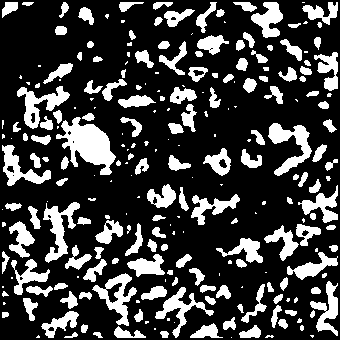
\includegraphics[width=\linewidth]{figures/snow2d_raw.png}
  \put(-2.86 ,0){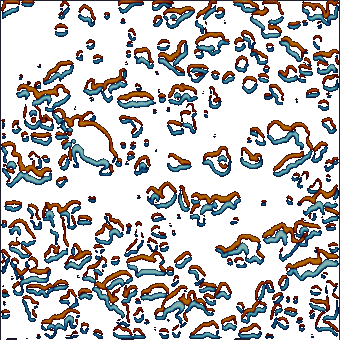
\includegraphics[width=\linewidth]{figures/diff_overlay.png}}
  \caption{}
  \label{fig:snow2d:diff}
\end{subfigure}
\hfill
\begin{subfigure}{0.53\linewidth}
  \includegraphics[width=\linewidth]{figures/snow2d_temp.pdf}
  \caption{}
  \label{fig:snow2d:grains}
\end{subfigure}
\caption{(a) The difference between the phase-field variable between initial and final simulations steps demonstrating where mass was gained (blue) and lost (orange) and (b) Tte difference in the ice grains initially (black) and after (white) 8 hours subjected to a \unitfrac[250]{K}{m} temperature gradient.}
\end{figure*}


\section{Yeti: Multi-scale Model}\label{sec:yeti}
The ability to develop a multi-scale model from existing MOOSE-based applications is a key feature for the framework allows for collaboration across scales and developers \citet{gaston2014physics}. Consider the two applications presented above---Pika and Ibex---that could easily be two modeling efforts underway at different institutions. This section demonstrates how the two models may be coupled together in a single application.

For this demonstration, a 2D Ibex simulation serves as the master application. This simulation is a 2D version of the solution presented in Section \ref{sec:ibex} with increased short-wave irradiance and reduced albedos to drive large temperature gradients for demonstration purposes. In this case rather than assuming a value of thermal conductivity it is computed using Pika. As illustrated in Fig. \ref{fig:yeti_flow}, Ibex computes the temperature and temperature gradient across the entire domain, then feeds these values to Pika application embedded at six locations, as shown in Fig. \ref{fig:yeti_keff}. Pika then evaluates and computes the effective thermal conductivity and returns that value back to Ibex for use for the next timestep.

\begin{figure}[b]
  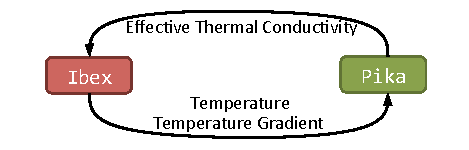
\includegraphics[width=\linewidth]{figures/flow.pdf}
  \caption{Flow chart showing information passing that occurs across scales.}
  \label{fig:yeti_flow}
\end{figure}

Each Pika simulation started from the same $\mu$-CT snow image and was fed temperature and temperature gradient information from Ibex and returned the effective thermal conductivity in the vertical direction, which was then linear interpolated accross the entire domain in the master Ibex application.  Fig. \ref{fig:yeti_keff} displays the change in temperature gradients that where passed to the Pika simulations and Fig. \ref{fig:yeti_keff} displays the change in thermal conductivity that is passed back to Ibex. Initially the $k_{eff}$ values were approximately \unitfrac[0.58]{W}{mK}. Note, this value differs from that values in Section \ref{sec:pika} due to using a larger interface thickness ($W$) to allow for a coarser finite element mesh to ease the computational requirements for the simulations.

\begin{figure*}

  \begin{subfigure}{0.49\linewidth}
    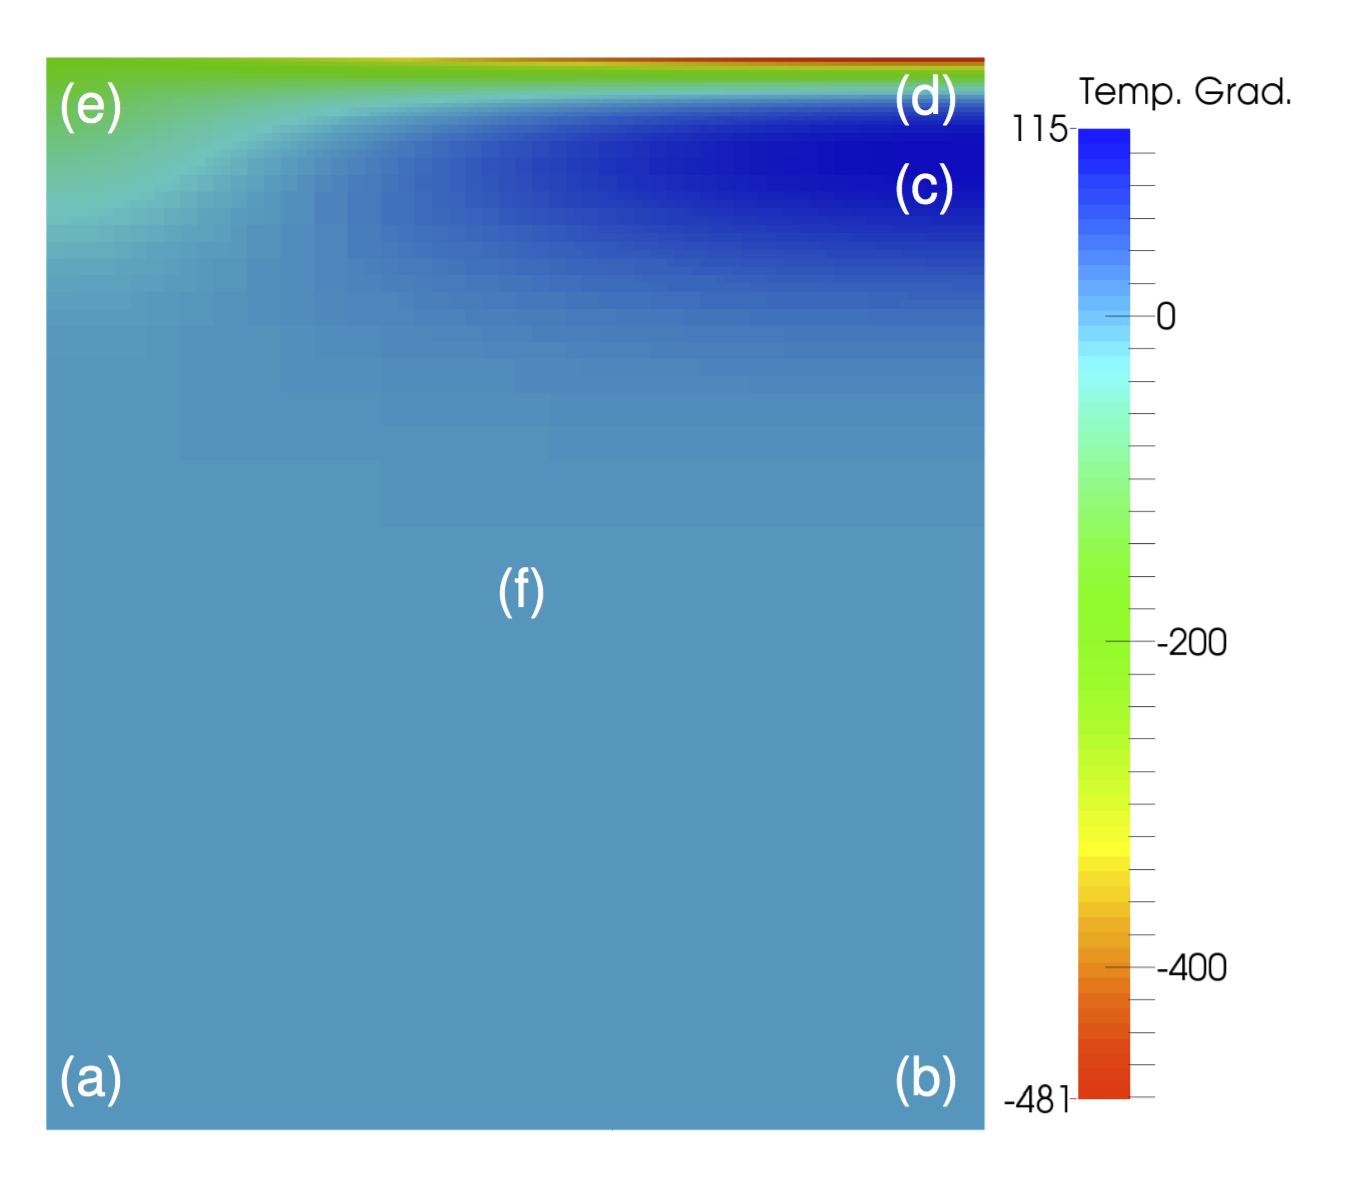
\includegraphics[width=\linewidth]{figures/yeti_TG.png}
    \begin{picture}(0,0)
      \put(0.1,0.3){\color{white}(a)}
      \put(2.15,0.3){\color{white}(b)}
      \put(2.15,2.49){\color{white}(c)}
      \put(2.15,2.69){\color{white}(d)}
      \put(0.1,2.69){\color{white}(e)}
      \put(1.175,1.5){\color{white}(f)}
    \end{picture}
    \caption{}
    \label{fig:yeti_TG}
  \end{subfigure}
  \hfill
  \begin{subfigure}{0.49\linewidth}
    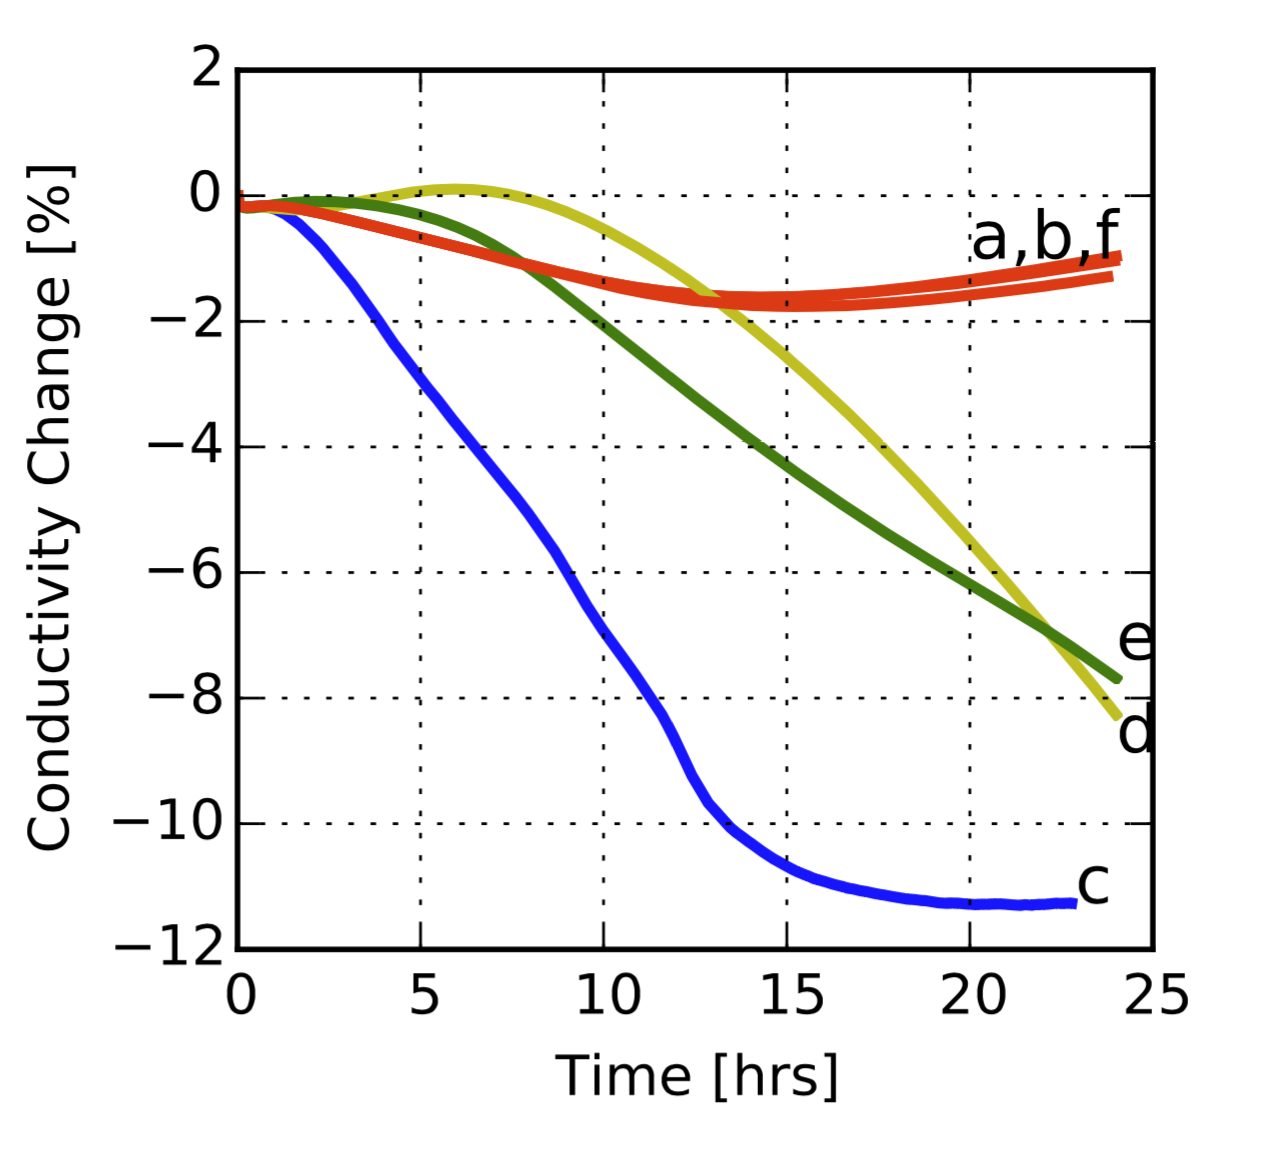
\includegraphics[width=\linewidth]{figures/yeti_keff.pdf}
    \caption{}
    \label{fig:yeti_keff}
  \end{subfigure}
  \caption{(a) Temperature gradient after four hours of simulation time and approximate locations of micro-structure Pika simulations and (b) the change in thermal conductivity as computed by the six Pika simulations.}
\end{figure*}

Refering to Fig. \ref{fig:yeti_keff}, the initial drop in conductivity is a result of the micro-structure simulation initializing to the supplied temperature gradient, whereas the results in Section \ref{sec:pika} started with an initialized temperature field. The area subjected to negative gradients (e and d) undergo changes resulting in constant or slightly increasing $k_{eff}$ and the location with a postive gradient, c, showed a decrease in conductivity. The points subject to zero gradient---a, b, and f---all behaved nearly identically and demonstrated a slight decrease in the conductivity, which may be a function of the phase-field method itself which tends to form circular geometries if not influenced by additional driving forces.

\begin{figure}[t]
  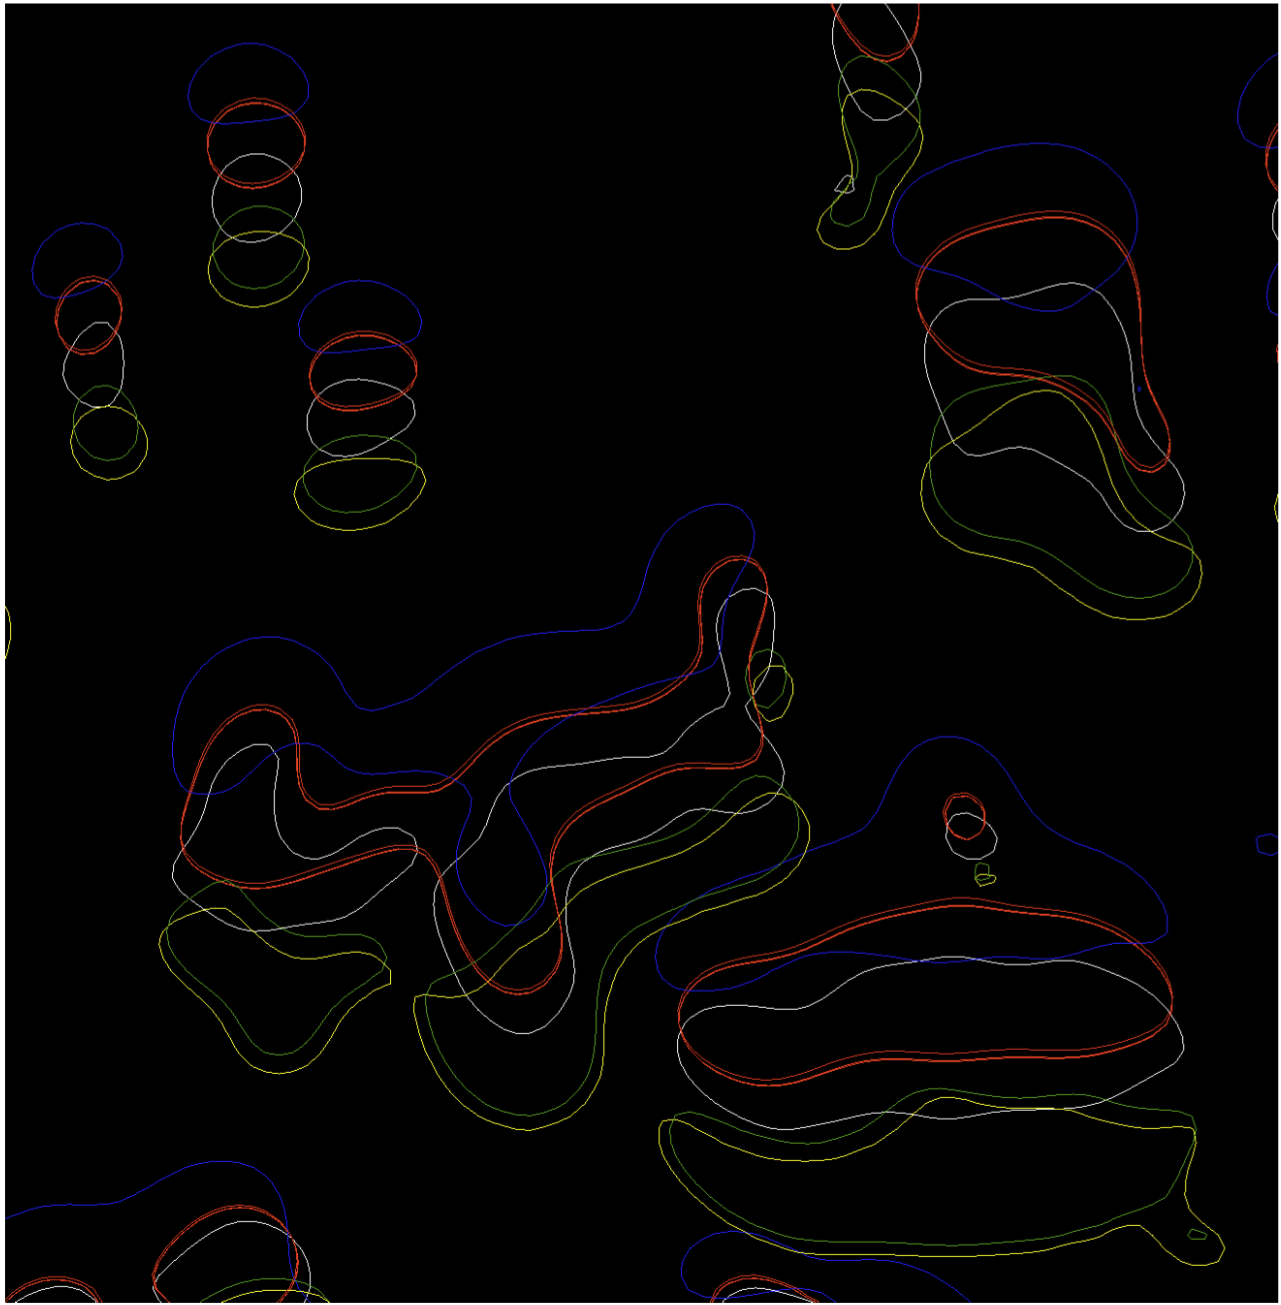
\includegraphics[width=\linewidth]{figures/yeti_micro_diff.pdf}
  \caption{Small sample of the changes in ice crystal shape from the initial condition (white) for the six Pika simulations: the colors match Fig. \ref{fig:yeti_keff} where simulations (a), (b), and (f) are red; (c) is blue; (d) is yellow; and (e) is green.}
  \label{fig:yeti_micro}
\end{figure}

Fig. \ref{fig:yeti_micro} shows the change in micro-structure between the various Pika simulations, the changes are in agreement with the results from the effecitve conductivity calculations and the temperature gradients the simulations were subjected. This figure only shows a small subset of the entire simulation to show detail. The initial condition, which was the same for all six simulations, is shown in white. The simulations without a gradient (a, b, and f) colored red all behaved nearly identical, but still showed movement that lead to changes in $k_{eff}$ larger than both areas with a postive gradient (e; green) and (d; yellow).

Again, due to the simplistic kinetics and method for computation of thermal conducivity exploring the reasons for the trends breify described here is not appropriate. Additionally, Pika includes temporal scaling parameters for various terms to make the numerical solution feasible, this was not considered in the meso-scale model and likely influenced the feedback between the models. However, as a pure demonstration of the capabilities offered by the MOOSE-framework, this result presents an example how two seperate applications, developed independantly, can be easily coupled together to build a multi-scale simulations.



\section{Closing Remarks}
The MOOSE framework is a powerful, finite element simulation framework capable of solving complex systems in a fully-coupled manner as evidenced by the growing number of MOOSE-base applications under development. The work presented here demonstrates the using MOOSE to model snow at differing scales is possible, and two applications where created as a starting point for future research: a meso-scale model for simulating snow as a continuum and a micro-structure model capable of tracking phase-change and ice grain boundaries. Using these two models a multi-scale simulation was performed to demonstrate the abilities to couple different applications together across scales.

The work performed aims to establish a new paradigm in snow and avalanche modeling: build a spectrum of applications using a common, open-source framework to allow access and ease of cross-development for researchers and practioners.



\section{Acknowledgments}
The submitted manuscript has been authored by a contractor of the
U.S. Government under Contract DE-AC07-05ID14517. Accordingly, the
U.S. Government retains a non-exclusive, royalty-free license to
publish or reproduce the published form of this contribution, or allow
others to do so, for U.S. Government purposes.
